\documentclass[11pt]{article}
\usepackage{fullpage}
\usepackage[utf8]{inputenc}
% \usepackage{algorithm}
% \usepackage{algorithmic}
\usepackage{amsfonts}
\usepackage{graphicx}
\usepackage{amsthm}
\usepackage{mathrsfs}
\usepackage{amssymb}
\usepackage{hyperref}
\usepackage{amsmath}
\usepackage{cite}
\usepackage{xcolor}
\newtheorem{theorem}{Theorem}
\newtheorem{lemma}{Lemma}
\newtheorem{definition}{Definition}
\newtheorem{claim}{Claim}
\newtheorem{corollary}{Corollary}
\newtheorem{observation}{Observation}
\newtheorem{remark}{Remark}
\newtheorem{oq}{Open Question}
\usepackage[normalem]{ulem}

% \usepackage{algorithm}
\usepackage{algpseudocode}
% \usepackage{aligned-overset}
% \usepackage{fontspec}
% \algrenewcommand\algorithmicrequire{\textbf{Precondition:}}
% \algrenewcommand\algorithmicensure{\textbf{Postcondition:}}
% \usepackage{xfrac}
% \usepackage{setspace}


\usepackage{algorithm}
\usepackage{algpseudocode}


% images
\usepackage{graphicx}
\graphicspath{ {./images/} }


\begin{document}
\title{Final Project - Distributed Graph Algorithms - Spring 2022\\
On the paper: "Can We Break Symmetry with $o(m)$ Communication?", by Shreyas Pai, Gopal Pandurangan, Sriram V. Pemmaraju, Peter Robinson
}
\author{Rotem Shavitt\footnote{rotemshavitt@campus.technion.ac.il, 209638162} \and Ido Frankel\footnote{ido.frankel@campus.technion.ac.il, 318985108}
}
\date{\today}
\maketitle

\section{Summary}

The article discusses the message complexity in distributed symmetry breaking problems, aiming specifically at $\Delta + 1 $ coloring and MIS problems. In global problems, it has been proven that $\Omega(m)$ messages are a lower bound with no additional assumptions. Knowing this, the authors are trying to answer whether this bound implies to local problems as well, or whether sublinear message complexity (i.e. $o(m)$) is possible for problems such as $\Delta +1$ coloring and MIS. The results are achieved in three different congest models, KT-1, KT-2 and the general model KT-$\rho$, (which stands for starting knowledge of neighbor's Ids till radius $\rho$).

\subsection*{Lower Bound}

The paper suggests 2 constructions of designated graphs in order to prove $\Omega(m)$ and $\Omega(n)$ lower bounds in KT-1 and KT-$\rho$ (for $\rho \ge 2$), respectively. 
\begin{figure}[h]
    \centering
    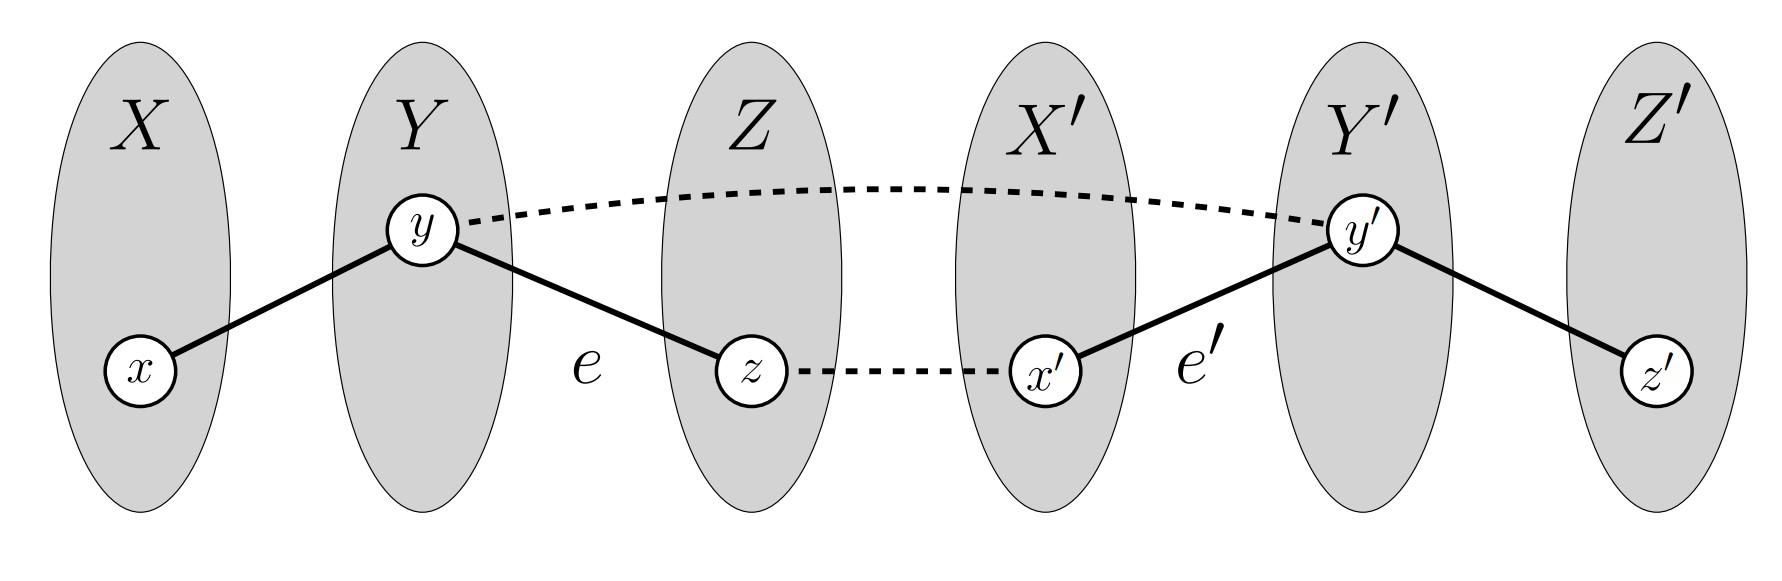
\includegraphics[scale=0.7]{graph_cross_graph}
    \caption{base graph $G \cup G'$, and the crossed graph $G_{e,e'}$}
    \label{fig:graph_cross_graph}
\end{figure}
First, the paper suggests a \textit{Base Graph} $G \cup G'$, where $G$ = $( X \cup Y \cup Z, E)$, in which $X \cup Y$, $Y \cup Z$ are complete bipartite graphs, and $G'$ is a copy of $G$. 
Then, we create a \textit{crossed graph} $G_{e,e}'$, as follows: 
We remove $e=(y,z)$ and $e'=(x',y')$ from the \textit{base graph}, and add $(z,x'), (y,y')$ which closes a cycle with $e,e'$. The authors then show that the previous graphs are similar in terms of executions for any comparison-base algorithm. They relies directly on the lemmas and definitions introduced by Awerbuch et al.\cite{Awerbuch}, which we will briefly introduce, In their paper they define an edge $(u,v)$ as utilized during an execution if a message is sent on it or if either $u, v$ sends or receives a message containing the other edge-end vertex ID assignment.

Awerbuch et al. showed that if pair of crossing edges $e, e'$ are not utilized during the execution by a comparison algorithm, then the executions of the touching nodes in both graphs are similar.

The article relies on the execution's similarities in order to show that by well-chosen edges in the graph, a contradiction can be achieved with respect to the correctness of problems such as $\Delta +1$ coloring and MIS. The contradiction then imposes a constraint on the comparison algorithm itself, which leads to the desired lower bounds.

In order to show the $\Omega(m)$ for the $(\Delta +1)$-coloring in KT$-1$ congest model, the authors suggest two different ID assignments $\phi, \psi$, for the base graph and the crossed graph, respectively. They then use the fact that $G$ and $G'$ are isomorphic in order to show that the execution $EX_G$ and $EX_{G'}$ are similar for every $v$ and $v'$. Later, based on the definition of $\psi$ the authors show that every vertex in $G$ and its counterpart in $G'$ have the same local state under $\psi$. Because $EX$ and $EX_{e,e'}$ are similar, it means that they have the same color. The contradiction is achieved by picking specific vertices $y,y'$ which are neighbours in the crossed graph, hence must not have the same color.

Next, the article proves a lower bound of $\Omega(n)$ in expectation w.h.p in the KT-$\rho$ model for any randomized Monte Carlo algorithm.
The proof presented in the article relies on previous work by by Linial \cite{Linial}, and Naor \cite{Naor} which present a lower bound on the rounds for any probabilistic algorithm for 3-coloring and MIS. The paper uses their results to present a lower bound of $\Omega(n)$ messages. It presents a graph $G$ consisting of a disjoint union of $\frac{n}{k}$ cycles (each of $k$ nodes, where $k$ is a constant defined in the paper). The authors assume by contradiction there exists an algorithm which sends sublinear amount of messages, since there are $\Omega(n)$ cycles, it holds that with high probability there exists a cycle which all of its nodes, do not send any message. Meaning, the output of such node is based on its initial knowledge which consists of the random choice of color, and its neighborhood. Because the behavior follows the same probability distribution under both KT-$\rho$ and KT-$0$, it implies that with high probability there exist two nodes in the cycle that produce the same color.

\subsection*{Upper Bound}
The article presents 3 new algorithms that improve message complexity under different circumstances. Two of them are for coloring problems and another for finding MIS.

\subsubsection*{Coloring}

The first algorithm presented uses the assumption of the KT-1 model and creates a $(\Delta+1)$ coloring solution in ${\Tilde{O}}(D+\sqrt{n})$ rounds with complexity of ${\Tilde{O}}(n^{1.5})$ messages. It is partitioning all vertices into $L, B_1, B_2, ..., B_k$ disjoint sets, and all color are divided into $C_1, C_2, ..., C_k$ uniformly. The Idea behind it is to run Johannson's \cite{Johansson} randomized coloring algorithm on a small enough partition in order to use only the corresponding color pallet. 

At first They Build a sparsified spanning subgraph $H$. Then, in each $B_i$ the nodes will execute a randomized algorithm for coloring by Johansson \cite{Johansson}. Then, until $G[L]$ has $\Tilde{O}(n)$ edges (which can be checked by using $H$), they recursively run the algorithm on $G[L]$ and finish.

The next algorithm shows how in the KT-1 CONGEST model when we drop the demand for $(\Delta+1)$ coloring solution and instead solve a $(1+\epsilon)\Delta$ coloring solution, we can improve message complexity to $\Tilde{O}(n/\epsilon^2)$. This algorithm works for any $\epsilon$ but is an improvement for higher values of $\epsilon$.
In each phase of the algorithm, every node chooses randomly a potential color, check if that choice is valid with respect to it's neighbors coloring, and if so determines it to be it's final color and deactivates. W.h.p, all the nodes are assigned a color after $O(\frac{\log{n}}{\epsilon})$ rounds. In each round, the active nodes needs to communicate with their active neighbors, counting to be $O((\log{n})^{2}/ \epsilon)$ w.h.p, summing into the message complexity $\Tilde{O}(n/\epsilon^2)$.

\subsubsection*{MIS}

The last algorithm presented in the article is an MIS algorithm that works in the KT-2 congest model. First, a set of $O(\sqrt{n})$ vertices is chosen as the starting input of a randomized greedy MIS algorithm. Each vertex $v$ that enters the MIS now needs to inform all $v$'s neighbors in order for them to deactivate themselves. In addition, we want to inform $v$'s 2-hop neighbors that their neighbors were deactivated. For this we use the additional knowledge of the KT-2 model. Because all the vertices of max distance 2 from $v$ know each other's IDs, they can calculate a BFS tree in $O(1)$. We use this tree to transfer messages instead of broadcasting which may cause a redundancy of messages sent. After the graph has been updated accordingly, they run Luby's \cite{Luby} algorithm on the remnant graph. In total, the message complexity achieved by this algorithm is $\Tilde{O}(n^{1.5})$.

To conclude, The article managed to prove that without additional assumptions to the knowledge of the KT-1 model, sublinear message complexity is not possible for $\Delta + 1$ coloring and MIS problems while using comparison-based algorithms. However, for non-comparison-based algorithm it presents a new coloring algorithm, which achieves sublinear message complexity. If we ease the problem into $(1+\epsilon)\Delta$ coloring, the article presents another non-comparison-based algorithm that achieves an even better message complexity (for certian $\epsilon$ values). For the MIS problem, by simply using the KT-2 model (instead of KT-1) the authors managed to compose an algorithm that reaches the desired sublinear message complexity.

\section{Suggested Questions}
\begin{enumerate}
    % \item If we use the KT-2 model assumption (or a different specific $\rho$ value), can we achieve a different upper bound for coloring.
    % \item Can we achieved better results under a specific graph family (for coloring or MIS).
    % \item Is there a certain assumption on $\Delta$ that can help achieve better results for coloring or MIS.
    \item What results can be achieved for $p$-defective $\Delta +1$ coloring in KT-1 CONGEST model.
    \item TODO - ROTEM - ADD RULING SET 
    
\end{enumerate}


\section{Related Work}
Most of the papers which discuss local problems that precede this article are revolved around round complexity bounds. Therefore, The results of the article are not an improvement of previous works, but a new angle for solving local problems.

On the other hand, there exist papers which discuss message complexity in global problems, one fundamental paper is of Awerbuch et al.\cite{Awerbuch} which showed that $\Omega(m)$ is a lower bound for broadcasting and spanning trees problems for comparison-based algorithms. In their paper Awerbuch et al. defined the terms of \textit{execution} of a protocol, and \textit{similarities} in order to show an equivalence between two algorithms. In addition the paper suggests a construction of a special family of network graphs (i.e. \textit{crossed graph}) for their lower bounds proof. Our paper pushed farther the construction of Awerbuch et al. and uses definitions which were initially defined in their paper in order to prove lower bounds in local problems.
Later, King et al. \cite{King} showed that by lifting the restriction of comparison-based algorithm, the lower bounds presented by Awerbuch et al. breaks. they further showed $\Tilde{O}(n)$ message complexity can be achieved for randomized non-comparison algorithms of such global problems.

\textbf{<TODO - Add Upper Bounds related work>}


% ======== PREVIOUS RELATED WORK (BY ROTEM) WHICH I DIDN'T KNOW HOW TO FIT. =============
% In this section we will elaborate the major algorithms which the paper is based on.
% The First algorithm presented in the upper bound section uses Johannson's \cite{johannson} and Luby's \cite{luby} randomized coloring algorithm. In both algorithms, each vertex keeps a list of colors which are not used by any of it's neighbors. Because the vertices doesn't know $\Delta$, the list is initialized to the first $d(v)+1$ colors. In each round, every vertex chooses a color randomly from it's pallet, then sends it to all neighbors. If there are no contradictions, it keeps it and informs all vertices in order for them to update their pallet accordingly. In Luby's algorithm there is an additional step of a coin flip to determine if a vertex will choose a color in this round.
% ======================================= 


\section{New Results}
Our efforts have been concentrated on modifying the paper's results to other interesting areas, such as $p$-defective $\Delta+1$-coloring, and $(k, k\log{n})$-ruling-Sets, which is a generalization of MIS [$(2,1)$-ruling set]. In sections ahead we will present an a modify algorithm that produces $p$-defective $\Delta+1$-coloring w.h.p with exchange of $O(n \frac{\log^3{n}}{\log^2{\frac{p-1}{2}}})$ messages, and \textbf{<TODO - COMPLTETE - RULING SET FINDING - ROTEM>}

\subsection{\texorpdfstring{p-defective $\Delta+1$-coloring using $O(n \frac{\log^3{n}}{\log^2{\frac{p-1}{2}}})$ messages in KT-1 Congest}{}}

\subsubsection*{Setting}
Similarly to shown in the article, At the beginning of the algorithm, one node generates \\ $C \cdot \log^2{n} \cdot \frac{\log{n}}{\log{\frac{p-1}{2}}}$ random bits and shares it with all other nodes using a  sparsified spanning subgraph of the original graph – called a danner \cite{Gmyr} using $\Tilde{O}(\frac{n}{\log{\frac{p-1}{2}}})$ messages and $\tilde{O}(n)$ rounds in the KT-1 Congest model, as shown in corollary 1.2 in our paper (\textbf{TODO, VERIFY ROUNDS AND MESSAGE COMPLEXITY, NOT SURE}). Each node $v$ that has not already permanently colored itself, will use random bit string $s_i$ (of length $\Theta(\log^2{n}$)) in Phase $i$ to first select a random hash function $h_i$ from a family of $\Theta(\log{n})$-wise independent hash functions $\mathcal{H}=\{h:[\text{poly}(n) \xrightarrow{} [\Delta+1] \}$. In lemma \ref{rounds} it is shown that our algorithm runs in $O(\frac{\log{n}}{\log{\frac{p-1}{2}}})$ rounds.

\begin{algorithm}
\caption{p-defective $\Delta+1$-coloring (One round)}
\begin{algorithmic}[1]
\State Each active vertex chooses a random $S_i$ string, and compute the corresponding $h_i(v.ID)$ candidate color from $\Delta+1$ color palette.
\State If less than $p$ of its neighbours have picked the same color, $v$ colors itself.

\If{v was colored}
    \State In any future round, $v$ must approve any of its neighbours coloring.
\Else
    \State go to step 1
\EndIf
\end{algorithmic}
\end{algorithm}

\begin{lemma}
\label{prob_pick_good_color}
Each vertex chooses a color, which was picked by at most $p-1$ of its neighbours with probability of $\frac{d}{(1+\Delta) \cdot p}$
\end{lemma}
For any of $v$'s neighbours (denote $d$ as the number of $v$'s neighbours), let $X_{u_i}$ be an indicator variable that indicates if neighbours $u_i$ has picked same color as $v$. Note $P(X_{u_i}) = \frac{1}{1 + \Delta}$. Let $X_v = \sum{X_{u_i}}$. By Markov's inequality $P(X_v \ge p) \le \frac{E(X_v)}{p} = \frac{d}{(1+\Delta) \cdot p}$

% \pagebreak
\begin{lemma}
\label{rounds}
A vertex successfully colors itself in $O(\frac{\log{n}}{\log{\frac{p-1}{2}}})$ rounds w.h.p
\end{lemma}

\begin{gather*}
P(v \text{ hasn't been color in round } i)\\ 
= P([v \text{ has at least p neighbours with same color as his }] \bigcup \; [\exists u\in N(v): c(v)=c(u) \land u \text{ rejects}]) \\
\underset{\text{Inclusion–exclusion}}{=} P(\underset{A}{\underbrace{x_v \ge p}}) + P(\underset{B}{\underbrace{\exists u\in N(v): c(v)=c(u) \land u \text{ rejects}}}) - P(A \bigcap B) \le P(A) + P(B) \\
= P(\underset{A}{\underbrace{x_v \ge p}}) + P(\overset{B}{\overbrace{\bigcup_{u \in N(v)} c(v)=c(u) \land u \text{ rejects}}}) \\
\underset{\text{U.B}}{\underbrace{\le}} P(x_v \ge p) + \sum_{u \in N(v)}{P(c(v)=c(u) \land x_u \ge p)} \\
=  P(x_v \ge p) + \sum_{u \in N(v)}{P(c(v)=c(u)) \cdot P(X_u \ge p \mid c(u) = c(v))} \\
= P(x_v \ge p) + \sum_{u \in N(v)}{\frac{1}{1 + \Delta} \cdot \frac{d_{u}-1}{(1+ \Delta) \cdot (p-1)} }
\end{gather*}

\begin{gather*}
\le \frac{\Delta}{(\Delta + 1) \cdot p} + \sum_{u \in N(v)}{\frac{1}{1 + \Delta} \cdot \frac{\Delta-1}{(1+ \Delta) \cdot (p-1)} } \\
\le \frac{\Delta}{(\Delta + 1) \cdot p} + \frac{\Delta^2}{(1 + \Delta)^2 \cdot (p-1)}
\le \frac{1}{p} + \frac{1}{p-1} \le \frac{2p}{p(p-1)} = \frac{1}{\frac{p-1}{2}}
\end{gather*}
Thus, the probability that $v$ does not color itself in $O(\frac{\log{n}}{\log{\frac{p-1}{2}}})$ rounds is:

\begin{gather*}
P(v \text{ wasn't been color during the entire algorithm}) \\ 
\le [(\frac{p-1}{2})^{-1}]^{c \cdot \frac{\log{n}}{\log{\frac{p-1}{2}}}}
= [(\frac{p-1}{2})^{-1}]^{\log_{\frac{p-1}{2}}{n^c}}= n^{-c} \\
P(\exists v \text{ which hasn't been colored}) = P(\bigcup_{i} v_i \text{ has not been colored}) \\
\underset{U.B}{\underbrace{\le}} \sum_{i}^{n} P(v_i \text{ hasn't been colored}) = n \cdot n^{-c} = n^{1-c} \\
\end{gather*}

Thus, the probability that all vertices have been colored is
\begin{gather*}
P(\textbf{all vertices have been colored}) = 1 - n^{1-c} = 1 - \frac{1}{n^{c-1}} = 1 - \frac{1}{n^{c'}}
\end{gather*}
Hence w.h.p all vertices have been colored in  $O(\frac{\log{n}}{\log{\frac{p-1}{2}}})$ rounds. 

\begin{lemma}
\label{colors_conflict}
There are at most $\log{n}$ vertices which could have picked same color $c$ as $v$ in every round.
\end{lemma}
In step 2, a vertex will check if less than $p$ of its neighbours have picked same color as itself, it will only check neighbours that could have chosen this color in this round or in any previous rounds. Because each vertex chooses hash function $h_i$ according to the corresponding $s_i$ (which is shared by all vertices, as described in the settings), under $KT-1$ congest model, each vertex knows its neighbours ID, hence it can locally calculates which of its neighbours could have picked same color as itself.

By Lemma \ref{prob_pick_good_color}, $E(x) = \frac{d}{1 + \Delta}$. Since the colors of the vertices are chosen using an $\Theta(\log{n})$-wise independent family of hash functions $\mathcal{H}$, then the indicators $X_{u_i}$, themselves (which represents whether a neighbour has picked same color $c$ as $v$) are $\Theta(\log{n})$-wise independent. By lemma A.2 from our paper's appendix, it holds w.h.p there are at most $O(\log{n})$ neighbours of $v$ which could have picked the same color $c$ as $v$ in this round.


\begin{lemma}
\label{message_per_round}
In each round, each vertex exchanges $O(\frac{\log^2{n}}{\log{\frac{p-1}{2}}})$ messages.
\end{lemma}
By lemma \ref{colors_conflict}, in each round, $v$ can have a conflict with $O(\log{n})$ of its neighbours. Hence $v$ has to check all of its $O(\log{n})$ neighbours which have chosen color $c$ in this round or prior rounds \textbf{WHY, ALSO PRIOR ROUND MAKE SURE THE CORRECTION OF THE ALGORITHM STILL HOLDS, IF TAKING INTO ACCOUNT PREVIOUS ROUNDS} to be sure that there isn't a situation where more than $p$ of its neighbours have picked same color as $c$ in same round. Since there are $O(\frac{\log{n}}{\log{\frac{p-1}{2}}})$ rounds w.h.p (according to lemma \ref{rounds}), color $c$ is chosen by only $O(\frac{\log^2{n}}{\log{\frac{p-1}{2}}})$ neighbours w.h.p during the algorithm.

\begin{lemma}
The algorithm exchanges $O(n\cdot \frac{\log^3{n}}{\log{\frac{p-1}{2}}})$ messages
\end{lemma}
By lemma \ref{message_per_round}, each vertex exchanges $O(\frac{\log^2{n}}{\log{\frac{p-1}{2}}})$ messages per round, By lemma \ref{rounds}, there are $O(\frac{\log{n}}{\log{\frac{p-1}{2}}})$ rounds w.h.p. Hence the total message complexity (for all vertices) is $O(n\cdot \frac{\log^3{n}}{\log^2{\frac{p-1}{2}}})$
\newpage

\bibliographystyle{alpha}
\bibliography{bib-filename}

\begin{thebibliography}{9}
\bibitem{Awerbuch}
Baruch Awerbuch, Oded Goldreich, David Peleg, and Ronen Vainish. 1988. A Tradeoff between Information and Communication in Broadcast
Protocols. 319 LNCS, 2 (1988), 369–379. https://doi.org/10.1007/BFb0040404

\bibitem{Linial}
Nathan Linial. 1992. Locality in Distributed Graph Algorithms. SIAM J. Comput. 21, 1 (1992), 193–201. https://doi.org/10.1137/02210

\bibitem{Naor}
Moni Naor. 1991. A Lower Bound on Probabilistic Algorithms for Distributive Ring Coloring. SIAM J. Discret. Math. 4, 3 (1991), 409–412. https://doi.org/10.1137/0404036

\bibitem{Johansson}
Ojvind Johansson. 1999. Simple Distributed ($\Delta$ + 1)-Coloring of Graphs. Information Processing Letters 70 70 (1999), 229–232.

\bibitem{Luby} Michael Luby. 1985. A Simple Parallel Algorithm for the Maximal Independent Set Problem. In Proceedings of the Seventeenth Annual ACM Symposium on Theory of Computing (STOC ’85). 1–10. https://doi.org/10.1145/22145.22146

\bibitem{King} Valerie King, Shay Kutten, and Mikkel Thorup. 2015. \href{https://doi.org/10.1145/2767386.2767405}{Construction and Impromptu Repair of an MST in a Distributed Network with o(m) Communication}

\bibitem{Gmyr}
Robert Gmyr and Gopal Pandurangan. 2018. \href{https://doi.org/10.4230/LIPIcs.DISC.2018.32}{Time-Message Trade-Offs in Distributed Algorithms}. In 32nd International Symposium on Distributed Computing, DISC 2018, New Orleans, LA, USA, October 15-19, 2018 (LIPIcs), Ulrich Schmid and Josef Widder (Eds.), Vol. 121. Schloss Dagstuhl-Leibniz-Zentrum für Informatik, 32:1–32:18. 
\end{thebibliography}
    

\end{document} 
